\section{Introduction: Transparent, Data-Driven Documents}

Making sense of and verifying data-driven claims is hard, even when the evidence base is open and accessible.
A key challenge lies in tracing specific claims back to the underlying data. In peer review, for example,
empirical claims typically lack author-supplied links to data, making them hard for reviewers to check
directly~\citep{weber20}. Paper retractions, meanwhile, are often attributable not to fraud, but to simple
errors in data management or analysis~\citep{hu25}. The use of large language models (LLMs) to interpret
scholarly documents has seen considerable attention recently, from fact-checking~\citep{abu-ahmad25} to
interpretation of charts and figures~\citep{roberts24}, but current LLM interfaces do not support direct
interrogation of visual or other outputs.

Recent work on data provenance and data visualisation~\citep{psallidas18smoke,bond25}, on the other hand,
takes a more infrastructural approach to tracing outputs back to data. These approaches link computed outputs
to their data sources directly, by tracking dependency information. This allows visual outputs to support
\emph{provenance queries}, user interactions (e.g. mousing over visual elements) that reveal how output
features relate to data. The advantage of this approach is that the relationships to data sources are exposed
automatically via trusted infrastructure, typically a query language or general-purpose programming language
which tracks how data flows through a computation. However, these approaches are limited to outputs computed
from data, such as visualisations. What is missing is a way to extend these ``direct interrogation'' features
to natural language itself, where the main claims of most scholarly articles are actually made.

In this paper, we address this gap by combining two complementary approaches: the ability of LLMs to
understand technical language and synthesise queries over data, plus the provenance-tracking infrastructure of
an open source programming language called Fluid (\url{https://f.luid.org/})~\citep{perera22,bond25}.
Together, these two technologies enable the creation of \emph{transparent documents}, web-based scholarly
articles with two key transparency features:
\begin{enumerate}
\item \textbf{Data-driven:} Quantitative statements expressed in natural language --- e.g.~that system $X$ is
faster than system $Y$ on some task --- are computed from the relevant data, rather than occurring
merely as static fragments of text.

\item \textbf{Data linking:} Readers and reviewers can interactively trace such claims back to the specific
data elements that support them, through embedded provenance queries.
\end{enumerate}

\figref{scigen-example-website}, generated from our implementation, illustrates these two features. The upper
section shows an excerpt from a research paper comparing text encoding techniques~\citep{zhang18}. When a
reader hovers over the phrase ``does not further improve'', the corresponding data entries are highlighted in
blue on the left. Other fragments (e.g. ``better than'', ``further improvements'') that refer to the same data
are also marked, allowing readers to explore supporting and contrasting evidence. The lower section shows a
counterfactual situation where we imagine the authors' experiments had produced different results: here the
phrase ``does not further improve'' is replaced by the ``further improves''. Transparent documents thus turn
static text into interactable, data-driven content able to expose the evidential basis of scholarly claims.

\begin{figure}%[h]
    \centering
    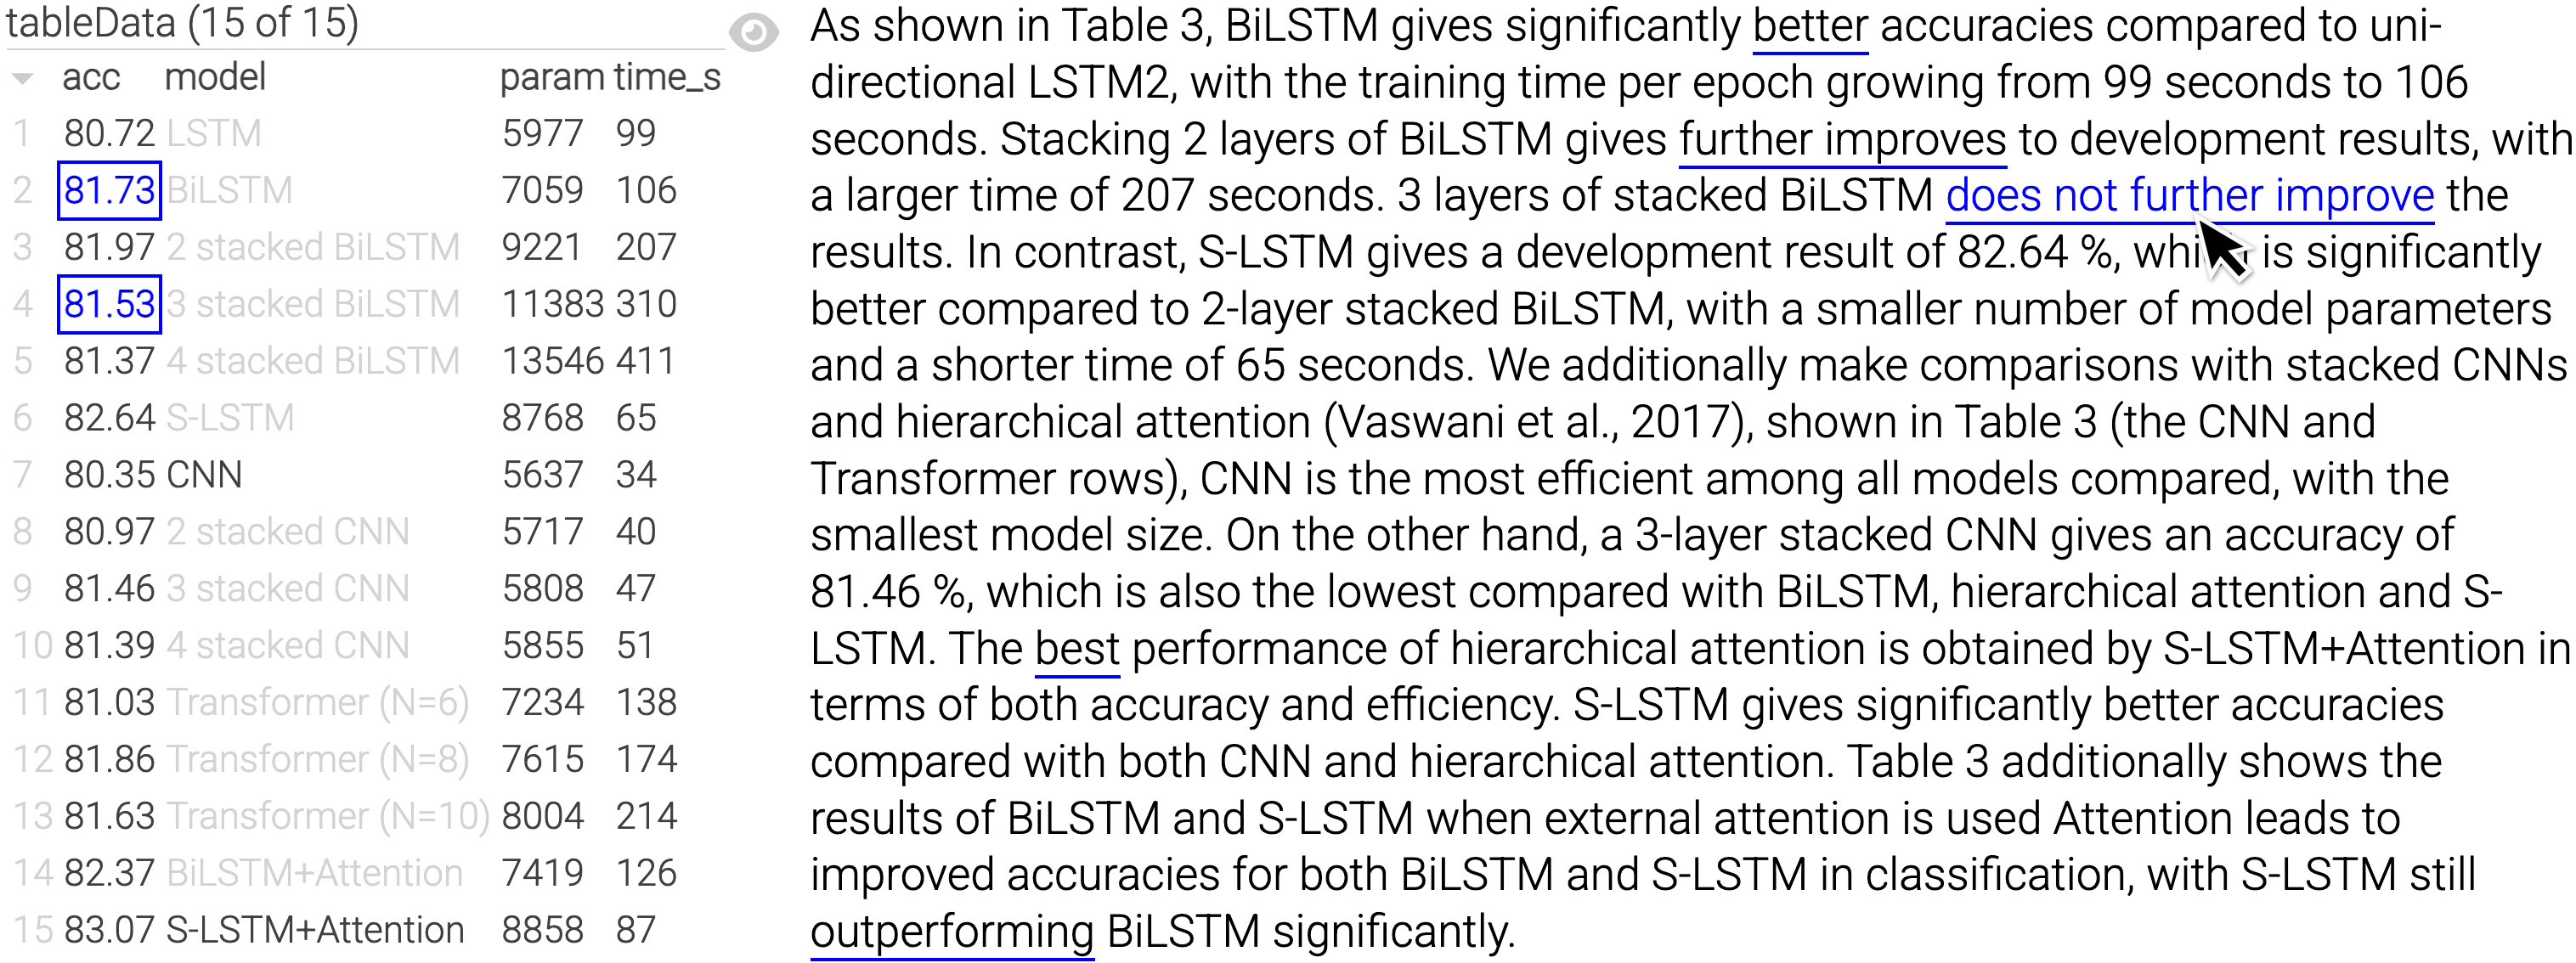
\includegraphics[width=\linewidth]{fig/scigen-1805.02474v1-10-with-pointer.png}
    \vspace{1mm}
    \hrule
    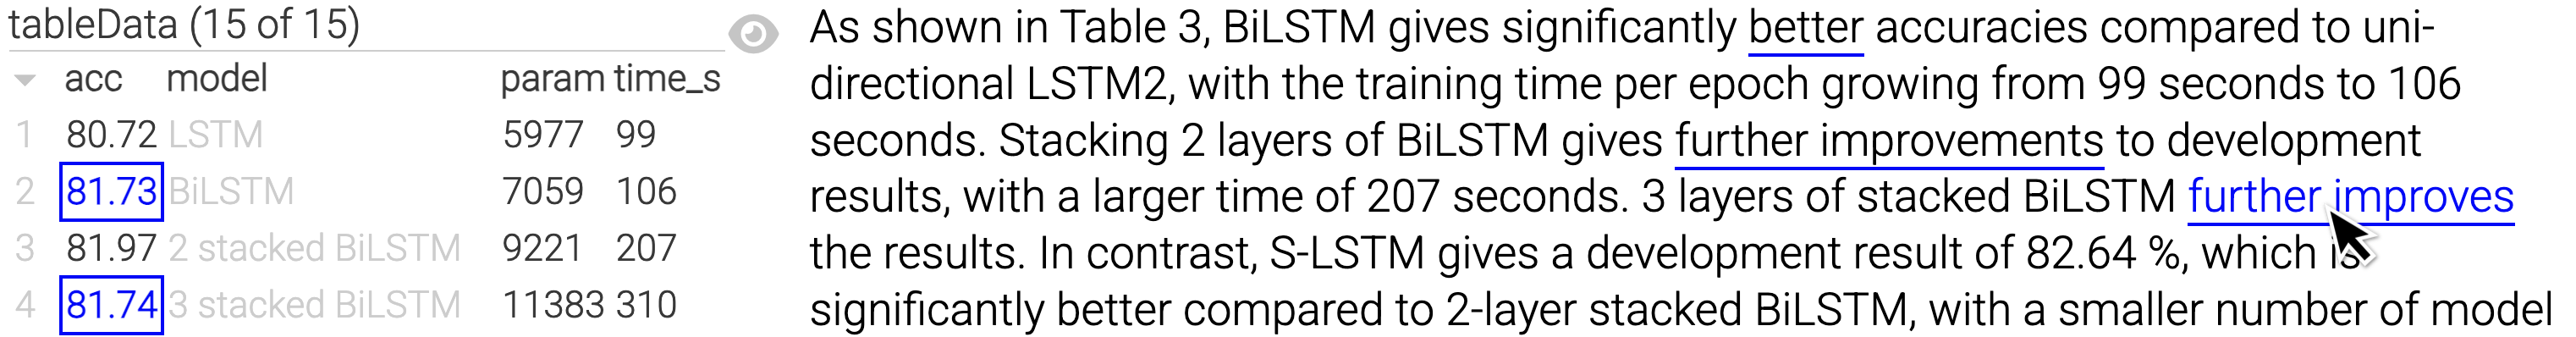
\includegraphics[width=\linewidth]{fig/scigen-1805.02474v1-10-counterfactual-with-pointer.png}
    \caption{\emph{Transparent document} example, showing data-driven natural language (top
    vs.~bottom)}
    \label{fig:scigen-example-website}
\end{figure}

\paragraph{Contributions.} Our specific contributions are:

\begin{itemize}
\item a proof-of-concept LLM-based tool for iteratively transforming a preexisting opaque document and
associated data set into a transparent, data-driven counterpart
\item an empirical evaluation of how well state-of-the-art models are able to solve the associated
interpretation and code synthesis problems
\end{itemize}

We leave implementing a full authoring plugin for an IDE such as VSCode or Cursor for future work.

We envisage two possible use cases for transparent text:

\begin{enumerate}
\item \textbf{Authoring.} Someone authoring content for an online article, wants to create text
linked to raw data (and derivative data such as charts or tabular summaries), so that the evidence base for
the claims made in the text can be explored \emph{in situ}, by interacting with the text.

\item \textbf{Reading or reviewing.} Someone reading textual claims derived from open data (e.g. a
scientific paper or climate report), wants to retroactively link the text to queries over the available data
and gradually ``rationally reconstruct'' the relationship between the claims in the paper and the evidence
base. Perhaps just to aid their own comprehension, or to provide some kind of justified peer review.
\end{enumerate}

\begin{figure}[h]
    \small
    % listings package seems to struggle, for now just use screenshot from VSCode
    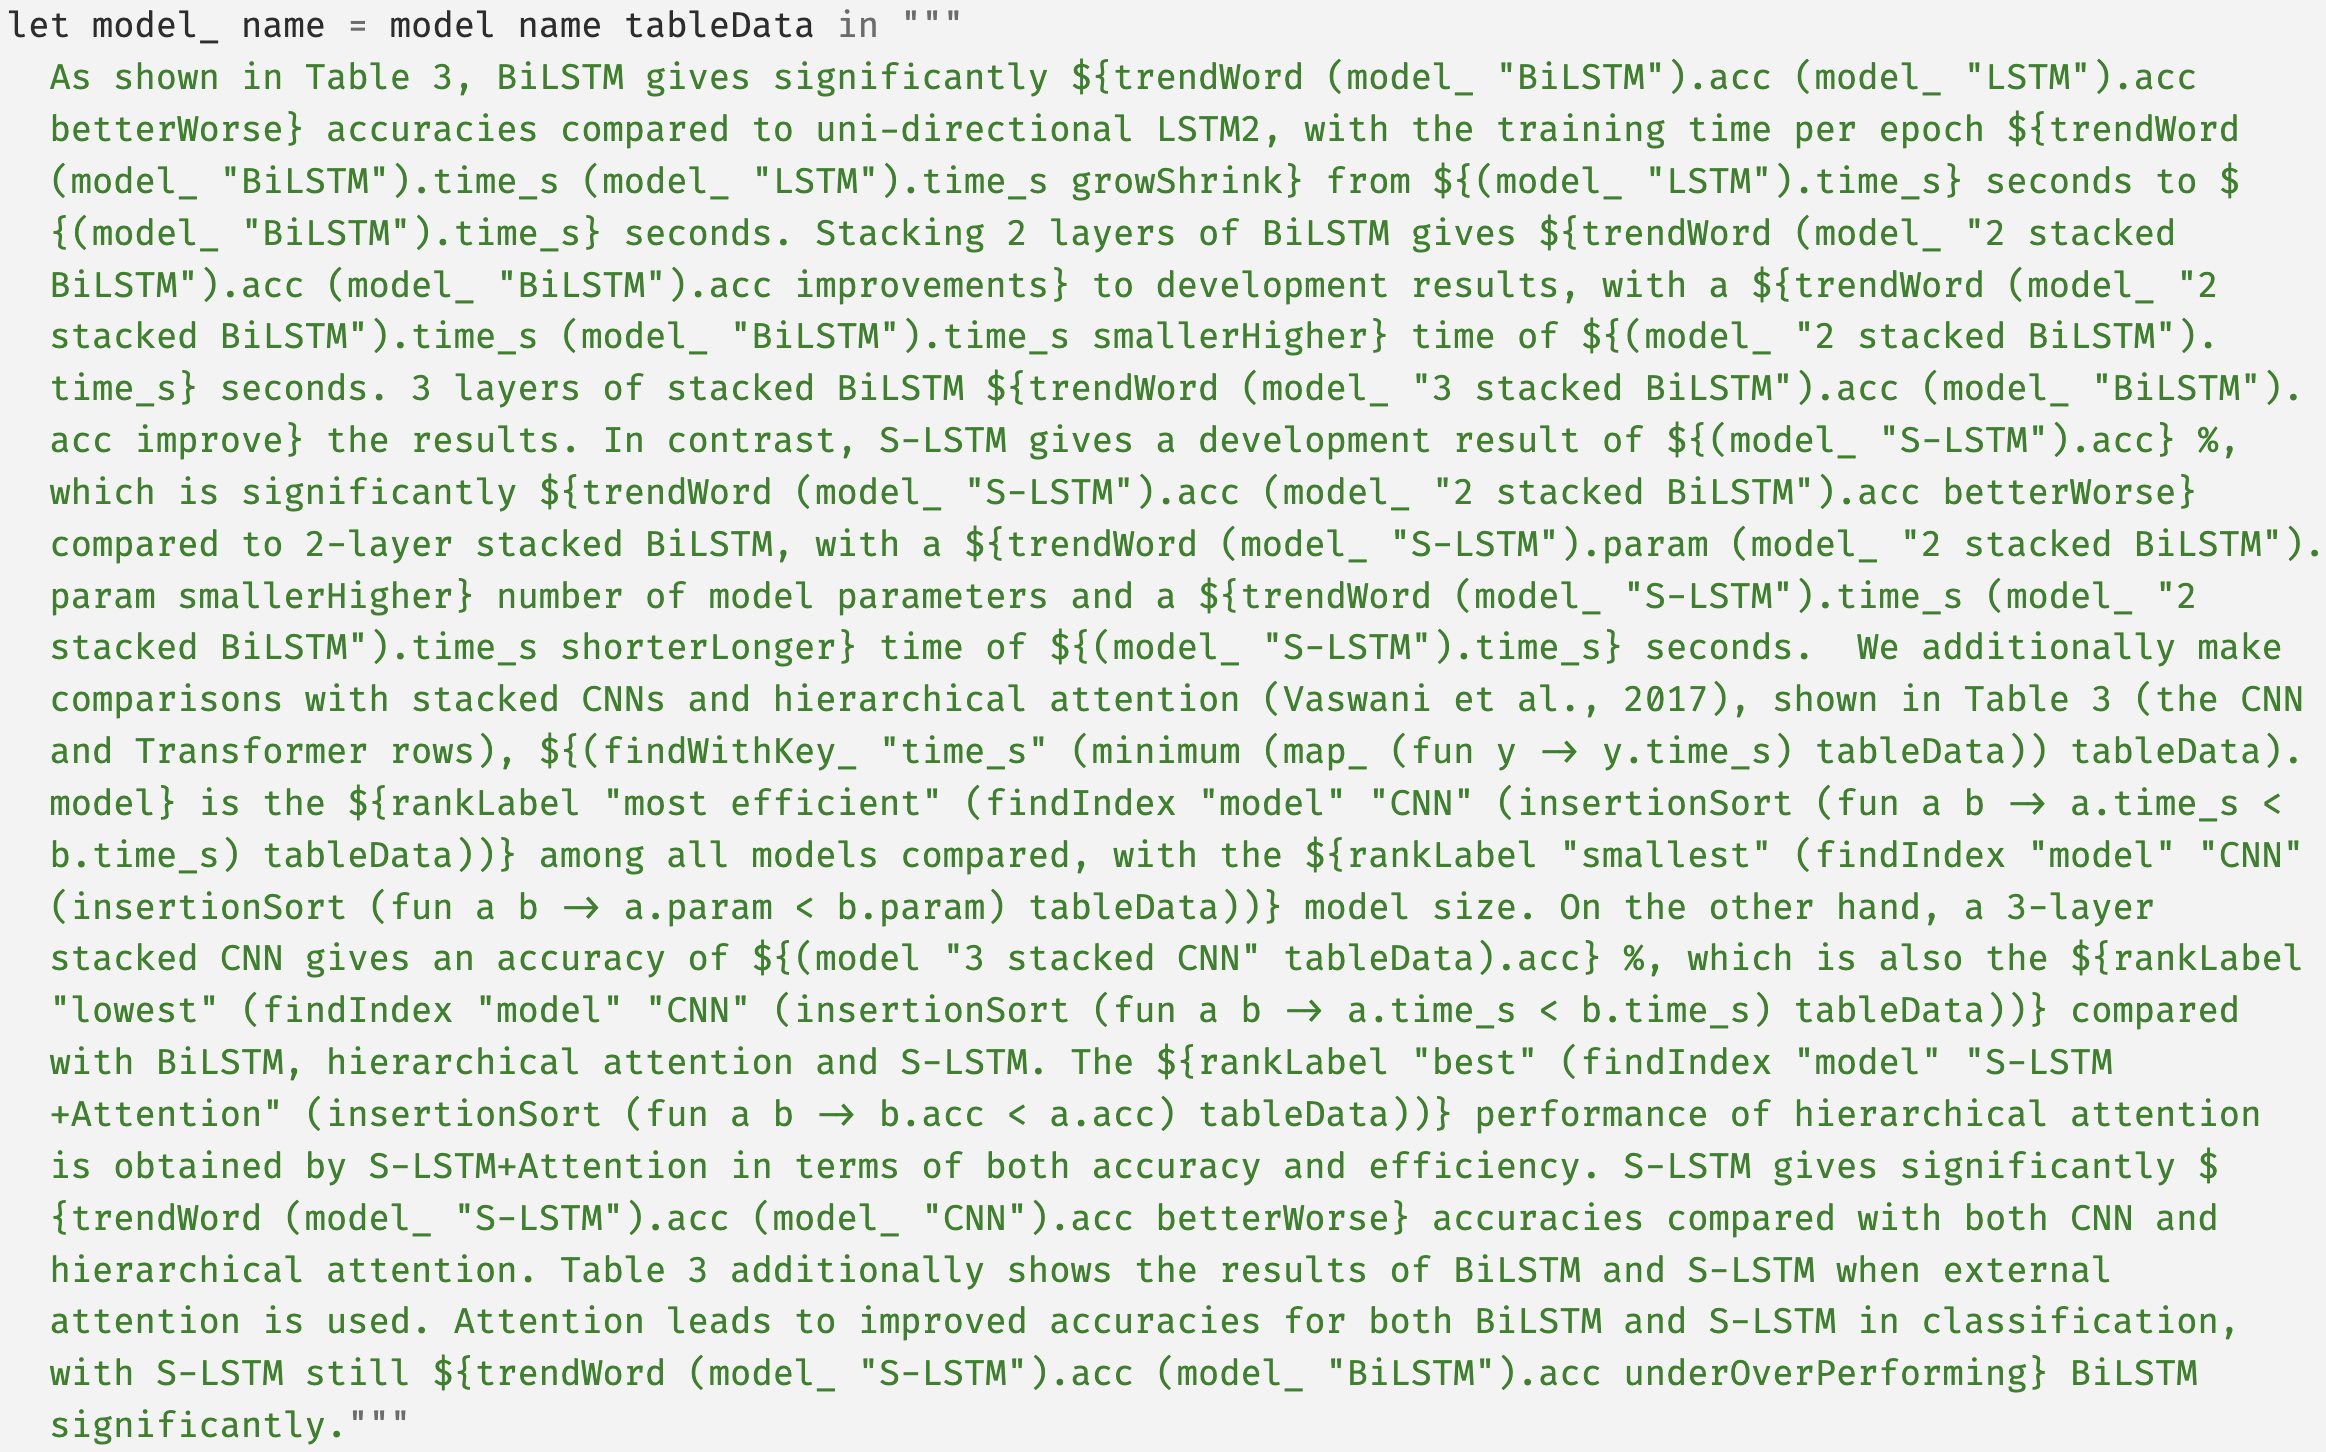
\includegraphics[scale=0.169]{fig/scigen-1805.02474v1-10-src-screenshot.png}
    \caption{Reference solution for transparent text in \figref{scigen-example-website}}
    \label{fig:fluid-example-paragraph}
\end{figure}


\subsection{Target idioms of natural language}

NLP aspect of the problem is potentially a big problem space in itself. We will restrict interest to certain
idiomatic uses of natural language in making/justifying scientific claims. Table~\ref{tab:fluid_examples}

\begin{table}[!ht]
    \centering
    \footnotesize
    \renewcommand{\arraystretch}{1.2}
    \begin{tabular}{>{\raggedright\arraybackslash}p{2cm} >{\raggedright\arraybackslash}p{5cm} >{\raggedright\arraybackslash}p{6cm}}
        \hline
        \textbf{Type}                & \textbf{Example} & \textbf{Generated Expression} \\
        \rowcolor{gray!20}
        \multicolumn{3}{>{\raggedright\arraybackslash}l}{\textbf{Quantitative expressions}} \\

        Numerical value
        & the training time per epoch growing from \hl{67} seconds to 106 seconds.
        &
        \begin{lstlisting}[language=Fluid,numbers=none]
(findWithKey' "model" "LSTM" tableData).time_s
        \end{lstlisting}
        \\
        Percentage &
        The Energy Sector accounts for total methane emissions of \hl{52.80\%} in 2030.
        &
        \begin{lstlisting}[language=Fluid,numbers=none]
(record.emissions /
 sum (map (fun x -> x.emissions)
          (getByYear year tableData))) * 100

        \end{lstlisting}  \\
        Rounding* & about 2 degrees warmer                & ~                             \\
        Cardinal* & three                & ~                             \\
        Multiplicative* & three times                & ~                             \\
        \rowcolor{gray!20}
        \multicolumn{3}{>{\raggedright\arraybackslash}l}{\textbf{Aggregation}} \\
        Average
        & The average methane emissions for the year 2030 is \hl{13.51} &
        \begin{lstlisting}[language=Fluid,numbers=none]
(sumEmissions year tableData / length records)
        \end{lstlisting} \\
        Min/Max                          & The Energy Sector recorded its highest methane emissions in \hl{2030}             &
        \begin{lstlisting}[language=Fluid,numbers=none]
let maxEntry =
    maximumBy (fun x -> x.emissions)
              (filter
                (fun x -> x.type == "Energy Sector")
                tableData)
in maxEntry.year
        \end{lstlisting} \\                             \\
        Rank &
        3-layer stacked CNN gives an accuracy of 81.46\%, which is the \hl{lowest} compared with BiLSTM, and S-LSTM  &
        \begin{lstlisting}[language=Fluid,numbers=none]
let pos =
  findIndex "model" "CNN"
    (insertionSort cmpTime tableData)
in rankLabel "lowest" pos \end{lstlisting} \\
        Total &
        The total methane emissions for the year 2030 is \hl{37.74} for Agriculture &
        \begin{lstlisting}[language=Fluid,numbers=none]
sumEmissions year tableData
        \end{lstlisting} \\
        Count*                       & ~                & ~                             \\
        \rowcolor{gray!20}
        \multicolumn{3}{>{\raggedright\arraybackslash}l}{\textbf{Trends}} \\

        Comparison
        & The training time per epoch \hl{growing} from 67 seconds to 106 seconds. &
        \begin{lstlisting}[language=Fluid,numbers=none]
trendWord
 (findWithKey' "model" "BiLSTM" tableData).time_s
 (findWithKey' "model" "LSTM" tableData).time_s
 growShrink
        \end{lstlisting} \\
        Graded adjective*            & \hl{extremely likely} to be exceeded in the 20th century               & ~                             \\
        Reference to visual element*                            & ~                & ~                             \\
        \hline
    \end{tabular}
    \caption{Quantitative/semi-quantitative natural language forms considered in this paper}
    \label{tab:fluid_examples}
\end{table}


\subsection{Contributions}

\begin{itemize}
    \item Design and proof-of-concept implementation of AI-assisted workflow for authoring transparent text
    (\secref{authoring-workflow})
    \item Empirical evaluation of how effective current LLMs are at providing the ``AI-assisted'' part
\end{itemize}
